% Copy this file to start a new note. Builds with pdflatex (the default recipe).
\documentclass[11pt]{article}
\usepackage{quicknotes}

\title{Data Science 6}
\author{Mark}
\date{}

\begin{document}
\maketitle

% \lecture{number}{date}{topic}
\lecture{3}{Monday, June 30, 2026}{Data, Variables and Arrays}

\section{Working with Data}
Consider social implications as data scinetist, power that comes with it to change. Yet also social implications can lead to pre-conceived notaions which change and restrict the model off the get go. 

\begin{figure}[h]
    \centering
    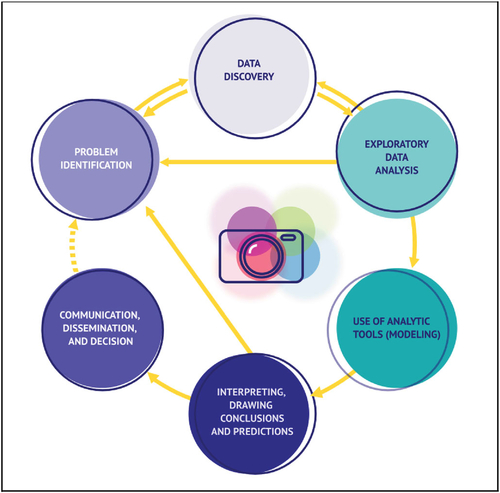
\includegraphics[width=0.7\textwidth]{image4.png}
    \caption{The life cycle of data science.}
    \label{fig:label}
\end{figure}
\section{Variables}
A \textbf{dataset} is a bunch of data gathered together. \textbf{tabular data} is jsut data with columns and rows, basically a table.
\textbf{Domain} is the set of possible values of a varaible. \textbf{Operationaliztion}: going from abstract data to having a vartiable and way to measure.
\newline
Ex: for a state population var domain is $\mathbb{Z}^{+}$. 
\newline
\begin{note}
    \itshape In python some people call python names variables but in this class variables differ from python names. 
\end{note}
\section{Variable Types}
Recall variable types from AP Stats. Numerical vs Categorical. Within numerical we have discrete and continous variables. Within categorial we have ordinal and nomial. Ordinal is simpley categories with inherent ordering. 

\begin{figure}[h]
    \centering
    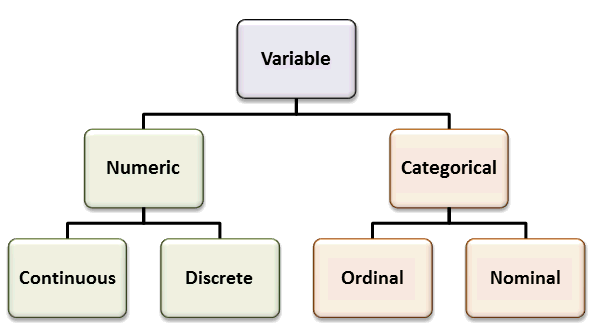
\includegraphics[width=0.7\textwidth]{image5.png}
    \caption{Diagram of var types}
    \label{fig:label}
\end{figure}

Ex: Area codes are categorical since you \textbf{can't do arithmetic with it}. 
\newline

\section{Units of Analysis}
\textbf{Units of analysis} is linked to the concept of vars because vars describe ceratin types of entities. Some examples are Indivualds, groups like families and variabels to understand that could be like income or num of people.

\section{Arrays}
Arrays are simply a data type where the name leads to a list of data types you can store in it. "A sequential collection of values".
Remember they are zero indexed, and same type in all array. Python artheimic are all element-wise operations.

\section{Numpy}



% Start typing. In math mode the snippets do the work:
% \[
%     \lim_{x \to 0} \frac{\sin x}{x} = 1
% \]

% \begin{definition}
% A function $f$ is continuous at $a$ if $\lim_{x \to a} f(x) = f(a)$.
% \end{definition}

% \begin{theorem}[Pythagoras]
% For a right triangle, $a^2 + b^2 = c^2$.
% \end{theorem}

\end{document}
